\chapter{10 Questions with a Real Estate Millionaire: Scale, Brokerage, and Contract Control}

This chapter reads the interview with Matt Teifke as a short lecture in commercial scale. We begin with the spectacle of a \(200{,}000\) dollar check and a first commission earned while still working at Papa John's, then move through the layered acquisition of real-estate knowledge, the institutional passage from agent to broker, the division of labor inside a partnership, and finally a worked wholesaling example. No validated board figures survive for this lecture, so the displayed mathematics below is a cautious reconstruction from the spoken record.

\section{Scale Shock and the First Commission}

We begin, as the interview begins, with money becoming concrete. The important point is not only that Teifke hears about large deals. He sees a local broker receive a check for \(200{,}000\), and this visual event reorganizes what the profession seems to permit. A second number then anchors the story at ground level: while still delivering pizza and mopping floors, he closes his first real-estate deal and remembers receiving roughly \(6{,}000\) to \(7{,}000\).

In these notes it is useful to put the scales next to one another:
\begin{align}
B_{\mathrm{observed}} &= 200{,}000, &
W_{\mathrm{ordinary}} &\approx 600, &
F_{\mathrm{first}} &\in [6{,}000,7{,}000].
\end{align}

The ratios are crude, but they explain the force of the anecdote:
\begin{equation}
\frac{F_{\mathrm{first}}}{W_{\mathrm{ordinary}}} \in [10,11.67],
\qquad
\frac{B_{\mathrm{observed}}}{W_{\mathrm{ordinary}}} \approx 333.
\end{equation}

The opening claim is therefore not mystical. It is a claim about unit scale. One successful real-estate event suddenly dominates many ordinary wage cycles.

\begin{remark}
The transcript gives both \(6{,}000\) and \(7{,}000\) for the first commission. It is safest to preserve this as a range rather than force a false precision.
\end{remark}

\section{Layered Formation and the College Question}

After the cold open, the interview resets and Teifke gives the long path by which he arrives at brokerage ownership. The order matters. We are not meant to see a single leap, but an accumulation of exposures:
\begin{itemize}
\item family influence through a mother who showed what real estate could make possible,
\item licensing at age \(17\),
\item work in a small brokerage,
\item commercial brokerage experience,
\item a master's degree in real estate with a financial emphasis,
\item apartment work and appraisal licensing,
\item third-party property management up to roughly \(700\) doors,
\item sale of that company,
\item construction of an entrepreneurial brokerage with Alex Kaufman.
\end{itemize}

The interview then asks whether college is necessary. Teifke's answer is structurally important. He does not say that institutional education is the decisive credential. He says, in effect, that it is an environment whose value depends on how aggressively one uses it. A classroom full of people interested in business is, on this view, a latent coordination device. The mechanism is not certification alone; it is opportunity density.

This section should therefore be read as preparation for the more technical beats that follow. The speaker has touched many layers of the stack, and when he later speaks about licensing, splits, and wholesaling, those claims rest on accumulated practice rather than on abstract advice.

\section{Entering the Market}

The interview then rewinds. This is the right move narratively, because the earlier biography gives us the outline but not the decisive scene in which a beginner first discovers how the market actually behaves.

Teifke describes showing up to brokerage interviews in a suit and tie, hoping to be granted a job. The conceptual reversal is that the market is not organized the way the novice imagines it. In his telling, brokerages want new agents. The beginner does not yet understand the demand structure of the profession.

\subsection{Question \& Answer}

\paragraph{Question.} How does a young agent actually break in?

\paragraph{Answer.} One first misidentifies the situation. The novice thinks he is pleading for admission, while the brokerage often wants fresh agents. What completes the transition is not merely getting hired; it is seeing the profession at full scale and then experiencing a first payout personally. The \(200{,}000\) dollar check provides the external proof. The first commission, received while he is still working an ordinary job, provides the internal proof. After that, the vocation no longer looks hypothetical.

This is why the Papa John's episode matters. The phone call comes while he is mopping the floor, and the first commission does not merely add income. It changes what work now seems worth organizing one's life around.

\section{From Agent to Broker}

The next question is institutional rather than autobiographical: once one is an agent, how does one move toward owning or operating a brokerage?

Teifke gives the answer in threshold form. Every agent must hang a license under a broker. Broker status is then governed by time, transaction history, and coursework. The important point is that the threshold moved during his own career.
\begin{align}
y_{\mathrm{broker,old}} &\ge 2,
&
y_{\mathrm{broker,now}} &\ge 4,
&
N_{\mathrm{pts}} &\gtrsim 900.
\end{align}

The points threshold is reported conversationally, so we should treat it as approximate. But even at that level of approximation, the structure is clear: broker status is not simply a matter of desire; it is a constrained progression through time, deal count, and educational requirements.

Once the license is in place, Teifke describes the economics of his current brokerage versus his first one. Let \(C\) denote a gross commission on a closed deal. Then the split rules are:
\begin{align}
C_{\mathrm{agent}} &= 0.9C, &
C_{\mathrm{firm}} &= 0.1C, \\
C_{\mathrm{agent,old}} &= 0.5C, &
C_{\mathrm{firm,old}} &= 0.5C.
\end{align}

The agent-side difference is immediate:
\begin{align}
C_{\mathrm{agent}} - C_{\mathrm{agent,old}}
&= 0.9C - 0.5C \\
&= 0.4C.
\end{align}

For a concrete example, if \(C=10{,}000\), then
\begin{equation}
C_{\mathrm{agent}} = 9{,}000,
\qquad
C_{\mathrm{agent,old}} = 5{,}000,
\qquad
C_{\mathrm{agent}} - C_{\mathrm{agent,old}} = 4{,}000.
\end{equation}

\begin{table}[h]
\centering
\caption{Commission split structures described in the interview}
\begin{tabular}{|c|c|c|}
\hline
Structure & Agent share & Firm share \\
\hline
Current brokerage & \(90\%\) & \(10\%\) \\
First brokerage & \(50\%\) & \(50\%\) \\
\hline
\end{tabular}
\end{table}

The institutional progression then ends in a moral progression. In the speaker's description, the broker becomes the one on the hook: the one responsible, the one who trains, and the one who supports the agents. That point matters because it turns a licensing threshold into a leadership burden.

\begin{remark}
The reported \(900\)-point threshold is not presented in the interview as a formally verified regulation. It should remain a speaker-reported approximation in the final notes.
\end{remark}

\section{Leadership and Partnership Design}

The interview next asks about the hardest part of owning a brokerage. The answer is not a formula but a control problem. One must continue to lead while deals fall apart, complaints accumulate, and lawsuits appear. The leadership task is thus not merely to optimize under good conditions, but to preserve operational steadiness under stress.

This leads naturally into partnership. Teifke gives a rough base-rate claim that very few partnerships work, then narrates why this one did. The essential mechanism is not sentiment. It is repeated testing, observation, and role differentiation.

We may schematize the division of labor as follows:
\begin{table}[h]
\centering
\caption{Functional split inside the partnership, as described in the interview}
\begin{tabular}{|c|c|}
\hline
Alex & Matt Teifke \\
\hline
operations & networking \\
profitability & relationship building \\
hiring and firing & new ideas \\
money discipline & outward growth \\
\hline
\end{tabular}
\end{table}

The vocabulary used late in the segment comes from entrepreneurial operating language: one partner is the implementer, the other the visionary. The notes should keep that phrase, but it should be understood as a functional split, not as branding. The mathematical content here is minimal, yet the structural content is substantial: the partnership survives because labor is partitioned rather than duplicated.

\section{Biggest Deal: Wholesaling as Contract Control}

We now come to the most explicit commercial arithmetic in the interview. The speaker names his biggest deal, then the interviewer asks for a quick explanation of wholesaling. This is a real teaching moment, and it deserves to be preserved carefully.

\begin{definition}
In the usage of this interview, wholesaling is the business of putting a property under contract, posting the money required to control that contract, and then monetizing that contract after finding a higher-value buyer. The crucial object is not merely the land itself, but the paper that gives control over the deal.
\end{definition}

\subsection{Question \& Answer}

\paragraph{Question.} What, exactly, is being sold in wholesaling?

\paragraph{Answer.} The interview presents the answer in a compressed but clear way: one first acquires contractual control. One then searches for a builder, developer, or other buyer willing to pay more. The economic asset is therefore the controlled right to complete or transfer the transaction. The property matters, of course, but the operative instrument is the contract.

The numerical data given in the interview are:
\begin{align}
P_0 &= 2.0\ \mathrm{M},
&
P_1 &= 2.7\ \mathrm{M},
&
\Delta P &= P_1 - P_0 = 0.7\ \mathrm{M}, \\
K_0 &= E+O \approx 20{,}000,
&
F_{\mathrm{wholesale}} &\in [700{,}000,780{,}000],
&
C_{\mathrm{broker}} &= 0.03P.
\end{align}

Here \(P_0\) is the contract price, \(P_1\) is the later buyer's offer, \(K_0\) is the earnest-plus-option money needed to control the contract, \(F_{\mathrm{wholesale}}\) is the assignment or wholesale fee stated in the interview, and \(C_{\mathrm{broker}}\) is the additional commission term the speaker says also went to their side.

The deal mechanics can be represented schematically.

\begin{figure}[h]
\centering
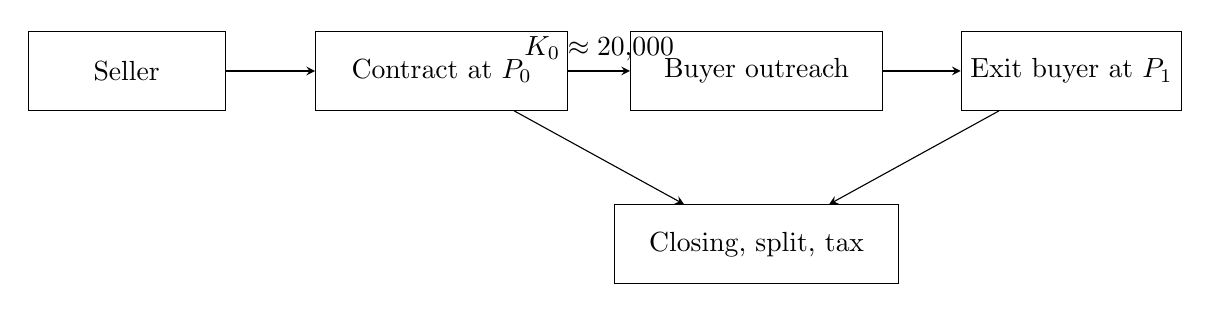
\begin{tikzpicture}[>=stealth]
\node[draw, rectangle, minimum width=2.5cm, minimum height=1cm] (seller) at (0,0) {Seller};
\node[draw, rectangle, minimum width=3.2cm, minimum height=1cm] (contract) at (4,0) {Contract at \(P_0\)};
\node[draw, rectangle, minimum width=3.2cm, minimum height=1cm] (outreach) at (8,0) {Buyer outreach};
\node[draw, rectangle, minimum width=2.8cm, minimum height=1cm] (buyer) at (12,0) {Exit buyer at \(P_1\)};
\node[draw, rectangle, minimum width=3.6cm, minimum height=1cm] (close) at (8,-2.2) {Closing, split, tax};
\draw[->] (seller) -- (contract);
\draw[->] (contract) -- node[above] {\(K_0 \approx 20{,}000\)} (outreach);
\draw[->] (outreach) -- (buyer);
\draw[->] (buyer) -- (close);
\draw[->] (contract) -- (close);
\end{tikzpicture}
\caption{Editorial reconstruction from the transcript: wholesaling as contract control, buyer search, and closing.}
\end{figure}

A cautious worked example then goes as follows.
\begin{enumerate}
\item Put the property under contract at \(P_0=2.0\ \mathrm{M}\).
\item Put up approximately \(K_0=20{,}000\) in earnest and option money to control the paper.
\item Search for builders, developers, and other buyers.
\item Receive an offer at \(P_1=2.7\ \mathrm{M}\).
\item Observe the spread \(\Delta P=0.7\ \mathrm{M}\).
\item Keep separate the stated wholesale fee \(F_{\mathrm{wholesale}}\) and the commission term \(C_{\mathrm{broker}}\).
\end{enumerate}

If, purely for illustration, we take the \(3\%\) commission to be computed on the \(2.0\ \mathrm{M}\) contract price, then
\begin{equation}
C_{\mathrm{broker}} \approx 0.03\times 2.0\ \mathrm{M} = 60{,}000.
\end{equation}

This gives a rough pre-tax gross pool
\begin{equation}
G \in [760{,}000,840{,}000],
\end{equation}
where the lower end uses \(700{,}000+60{,}000\) and the upper end uses \(780{,}000+60{,}000\).

If this pool is then split three ways before taxes, the pre-tax per-partner amount is
\begin{equation}
\frac{G}{3} \in [253{,}333,280{,}000].
\end{equation}

In a more symbolic form, letting \(T\) denote taxes and other reductions, we may summarize the reported logic by
\begin{equation}
N_{\mathrm{partner}} \approx \frac{F_{\mathrm{wholesale}} + C_{\mathrm{broker}} - T}{3}.
\end{equation}

The speaker's own caution is essential here. The headline number is not the net number. Taxes bite hard, and the interview insists that the visible gross should not be mistaken for disposable gain.

\begin{remark}
Two uncertainties must remain explicit. First, the transcript gives both \(700{,}000\) and \(780{,}000\) for the wholesale fee. Second, the base price \(P\) in the \(3\%\) commission term is not fully pinned down. The arithmetic above is therefore illustrative rather than exact.
\end{remark}

\section{Losses, Strange Events, and the Long Horizon}

After the biggest deal, the interview circles back to best and worst decisions. The worst decision is described as cannabis stock, with losses down multiple millions. The important feature of this segment is volatility. The speaker does not merely say that the investment performed poorly; he says the position can move by large five-figure amounts in a day.

A compact summary of the reported numbers is
\begin{equation}
|\Delta V_{\mathrm{cannabis,day}}| \in [60{,}000,100{,}000],
\qquad
R_Q \approx 67\ \mathrm{M},
\qquad
V_{\mathrm{equity}} \approx 40\ \mathrm{M}.
\end{equation}

These are the speaker's claims about revenue, valuation, and mark-to-market strain. The lecture does not turn them into a formal valuation proof, and neither should we. Their function is different: they show how large nominal wealth can coexist with daily discomfort, uncertainty, and drawdown.

The best decision, by contrast, is not presented as an asset purchase but as a partnership decision. This is consistent with the whole structure of the interview. A great deal, a great split, and even a great license matter, but the durable engine is the right operating partner attached to a clear goal.

The ``craziest story'' segment has a similar effect. On its surface it is anecdotal and bizarre: a pregnant wife chased by a woman with a stick and a dog, then an RV-park negotiation over beer. But structurally the point is simple. Real estate is messy, field-bound, and filled with situations that do not fit polished business imagery. The speaker presents this not as an exception, but as part of the normal texture of the work.

The final motivational section then returns to the geometry of long-term effort. The guiding idea is that clear goals organize the day-to-day burden. One keeps going not by remaining perpetually on fire, but by having a definite direction and by receiving repeated confirmation that the work changes other people's lives.

\section{Summary}

We can now see the interview's internal order. It begins with a change of scale, moves through accumulated exposure to the real-estate stack, rewinds to the first entry into the market, formalizes the passage from agent to broker, and then shows how partnership design and contract control generate large economic outcomes. Along the way, the lecture insists on a sober symmetry: big numbers are real, but so are taxes, failed deals, lawsuits, drawdowns, and the long patience required to keep building.

The mathematically useful content of the chapter is therefore modest but sharp. We retain the scale ratios of the opening, the threshold logic of broker licensing, the split formulas of brokerage economics, and the worked arithmetic of a wholesale deal. The broader lesson is that wealth here is not treated as magic. It is treated as a sequence of institutional positions, negotiated contracts, role divisions, and repeatedly tested judgments. That is the level at which the interview is most instructive.